% !TeX program = xelatex
\documentclass[a4paper,14pt,russian]{extreport}
% Оформление адаптировано из course-work-CG-BMSTU-5-sem.
\usepackage{iftex}
\ifPDFTeX
  \usepackage{cmap}
  \usepackage[T2A,T1]{fontenc}
  \usepackage[utf8]{inputenc}
  \renewcommand{\rmdefault}{Tempora-TLF}
\else
  \usepackage{fontspec}
  \IfFontExistsTF{Times New Roman}{\setmainfont{Times New Roman}}{\setmainfont{TeX Gyre Termes}}
  \IfFontExistsTF{Courier New}{\setmonofont{Courier New}}{\setmonofont{DejaVu Sans Mono}}
\fi
\usepackage[main=russian,english]{babel}
\usepackage[left=30mm,right=10mm,top=20mm,bottom=20mm]{geometry}
\usepackage{microtype}
\usepackage{setspace}
\onehalfspacing
\usepackage{indentfirst}
\setlength{\parindent}{12.5mm}
\setlength{\emergencystretch}{2em}
\clubpenalty=10000
\widowpenalty=10000
\usepackage{graphicx,float}
\usepackage{amsmath,amssymb}
\numberwithin{equation}{chapter}
\usepackage{tabularx,booktabs}
\usepackage{enumitem}
\setlist{topsep=4pt,itemsep=0pt,parsep=0pt}
\setlist[itemize]{label=---,leftmargin=\parindent}
\setlist[enumerate]{label=\arabic*),leftmargin=\parindent}
\usepackage{titlesec,tocloft}
\titleformat{\chapter}[block]{\large\bfseries\centering}{\thechapter}{0.5em}{}
\titleformat{\section}{\large\bfseries\raggedright}{\thesection}{0.5em}{}
\titleformat{\subsection}{\normalsize\bfseries\raggedright}{\thesubsection}{0.5em}{}
\titlespacing*{\chapter}{0pt}{-22pt}{14pt}
\titlespacing*{\section}{0pt}{12pt}{8pt}
\titlespacing*{\subsection}{0pt}{10pt}{6pt}
\setcounter{tocdepth}{2}
\setcounter{secnumdepth}{2}
\setlength{\cftbeforetoctitleskip}{-25pt}
\renewcommand{\cfttoctitlefont}{\large\bfseries}
\renewcommand{\cftchapleader}{\cftdotfill{\cftdotsep}}
\setlength{\cftbeforechapskip}{5pt}
\usepackage[singlelinecheck=false]{caption}
\DeclareCaptionLabelSeparator{emdash}{~---~}
\captionsetup{labelsep=emdash}
\captionsetup[figure]{justification=centering,name=Рисунок}
\captionsetup[table]{justification=raggedright}
\usepackage{csquotes}
\usepackage[backend=biber,style=gost-numeric,language=auto,sorting=none,maxnames=4,doi=false,isbn=false,url=true,dashed=false]{biblatex}
\addbibresource{ref-lib.bib}
\usepackage{xurl}
\urlstyle{same}
\usepackage[unicode,hidelinks]{hyperref}
\usepackage{bookmark}
\AtBeginBibliography{\small\singlespacing}
\setlength{\bibitemsep}{7pt}
\pagestyle{plain}

\hypersetup{
  pdftitle={Исследование нейросетевых методов обнаружения повторного JPEG-сжатия изображений},
  pdfauthor={Гиричев М. С.}
}
\begin{document}
\hypersetup{pageanchor=false}
\begin{titlepage}
\centering
\begin{minipage}{0.12\textwidth}
  
\includegraphics[width=\linewidth]{images/bmstu_logo_vector.pdf}
\end{minipage}\hfill
\begin{minipage}{0.85\textwidth}
  \centering\singlespacing\fontsize{10}{12}\selectfont\bfseries
  Министерство науки и высшего образования Российской Федерации\\
  Федеральное государственное автономное образовательное учреждение\\
  высшего образования\\
  «Московский государственный технический университет\\
  имени Н. Э. Баумана\\
  (национальный исследовательский университет)»\\
  (МГТУ им. Н. Э. Баумана)
\end{minipage}
\par\vspace{3mm}\hrule height 0.5pt
\vspace{1mm}\hrule height 1.5pt
\vspace{5mm}
\begin{flushleft}
\small\singlespacing
ФАКУЛЬТЕТ ИУ «Информатика и системы управления»\par\vspace{3mm}
КАФЕДРА ИУ7 «Программное обеспечение ЭВМ и информационные технологии»
\end{flushleft}
\vspace{19mm}
{\large\bfseries РАСЧЁТНО-ПОЯСНИТЕЛЬНАЯ ЗАПИСКА\par}
\vspace{6mm}
{\large\bfseries К КУРСОВОЙ РАБОТЕ\par}
\vspace{6mm}
по дисциплине\par
«Основы искусственных нейронных сетей»\par
\vspace{10mm}
{\large НА ТЕМУ:\par}
\vspace{5mm}
{\large Исследование нейросетевых методов обнаружения повторного JPEG-сжатия изображений\par}
\vfill
\begin{tabularx}{\textwidth}{@{}l l >{\centering\arraybackslash}X r@{}}
Студент & ИУ7-76Б & \rule{30mm}{0.4pt} & Гиричев М. С.\\[-2mm]
 & & {\scriptsize (подпись, дата)} & \\[5mm]
Руководитель & & \rule{30mm}{0.4pt} & Кудрявцев М. А.\\[-2mm]
 & & {\scriptsize (подпись, дата)} &
\end{tabularx}
\vspace{14mm}
\par Москва, 2026
\end{titlepage}

\setcounter{page}{2}
\hypersetup{pageanchor=true}
% Источник для редактирования бланка — assignment.docx.

\includepdf[pages=1,pagecommand={\thispagestyle{empty}}]{assignment.pdf}

\renewcommand{\contentsname}{\centerline{СОДЕРЖАНИЕ}}
\phantomsection
\pdfbookmark[0]{СОДЕРЖАНИЕ}{toc}
\tableofcontents
\chapter*{ВВЕДЕНИЕ}
\addcontentsline{toc}{chapter}{ВВЕДЕНИЕ}

При отборе фотографий для экспертного анализа специалисту нередко доступна только последняя JPEG-копия. Снимок могли сохранить при экспорте из редактора или при подготовке к публикации. Внешне две версии могут выглядеть одинаково, хотя второе сжатие изменило распределение частотных коэффициентов. По этим изменениям можно выделить часть повторно сохранённых файлов и передать их специалисту для дальнейшего анализа~\cite{wang2016,park2018}.

Цель работы --- разработать программу, которая обнаруживает признаки повторного JPEG-сжатия по одному файлу, и установить, как выбор нейросетевой модели влияет на качество классификации и время обработки изображения.

Для достижения цели поставлены следующие задачи.
\begin{enumerate}
  \item Сформулировать требования к программе и ограничения на входные изображения.
  \item Сравнить методы обнаружения повторного JPEG-сжатия и выбрать нейросетевые модели для исследования.
  \item Спроектировать структуру программы и алгоритмы подготовки данных, обучения и классификации.
  \item Выбрать средства реализации и разработать программу для обработки JPEG-файлов.
  \item Обучить модели на размеченном наборе однократно и двукратно сжатых изображений.
  \item Сопоставить ошибки и время обработки у двух моделей, определить влияние параметров первого и второго сжатия на результат.
\end{enumerate}

\chapter{Аналитический раздел}

\section{Постановка задачи}

JPEG-сжатие с потерями изменяет значения пикселей изображения. Если полученный файл декодировать и снова сохранить в JPEG, изображение пройдёт второй цикл сжатия. Следы этих операций могут использоваться при анализе истории обработки изображения. Повторное сохранение возможно и без изменения содержания снимка, поэтому обнаружение двукратного сжатия само по себе не доказывает наличие подделки.

В работе решается задача классификации JPEG-файла по числу выполненных сжатий. Рассматриваются два класса:
\begin{itemize}
  \item однократно сжатые изображения, полученные JPEG-кодированием исходных изображений без предшествующего JPEG-сжатия;
  \item двукратно сжатые изображения, полученные декодированием однократно сжатых изображений и их повторным JPEG-кодированием.
\end{itemize}

Входными данными служит только проверяемый JPEG-файл. Исходное несжатое изображение и параметры первого сжатия при проверке неизвестны. Выходными данными являются предсказанный класс и оценка модели для класса двукратного сжатия.

Область исследования ограничивается повторным сжатием с совпадающей сеткой блоков JPEG. Между сохранениями не выполняются масштабирование, поворот и смещение изображения. Предполагается, что всё изображение имеет общую историю сжатия. Локализация вставленных областей и определение точного числа сжатий, превышающего два, в задачу не входят.

\section{Признаки повторного JPEG-сжатия}

В режиме JPEG на основе дискретного косинусного преобразования (ДКП) компоненты изображения обрабатываются блоками размером $8\times8$ отсчётов. Каждый блок преобразуется в набор частотных коэффициентов, которые затем квантуются и кодируются~\cite{jpeg_standard}. Квантование уменьшает точность представления коэффициентов и создаёт основные потери информации.

Для отдельного коэффициента операция квантования записывается в виде
\begin{equation}
  k = \operatorname{round}\left(\frac{c}{q}\right),
\end{equation}
где $c$ --- коэффициент ДКП до квантования; $q$ --- соответствующий элемент таблицы квантования; $k$ --- целочисленный результат; $\operatorname{round}$ --- округление до ближайшего целого. При декодировании восстанавливается значение $kq$, которое в общем случае отличается от $c$.

После второго сжатия распределения коэффициентов могут приобретать дополнительные максимумы и пропуски значений. Эти закономерности зависят от таблиц первого и второго квантования. Для их описания используют гистограммы: для каждой выбранной частоты подсчитывается, как часто коэффициенты попадают в заданные интервалы~\cite{wang2016}. Нейронная сеть может обучаться различать такие распределения у двух классов изображений.

В JPEG-файле доступны таблицы квантования последнего сохранения. Они характеризуют условия получения наблюдаемого изображения и могут передаваться модели вместе с гистограммами~\cite{park2018}. Числовой параметр качества, задаваемый в графическом редакторе, служит способом выбора таблиц и не является универсальной характеристикой для всех программ кодирования.

Выраженность следов повторного сжатия неодинакова. При близких параметрах двух сохранений различия могут быть малы. Однородные области также содержат меньше частотной информации для классификации~\cite{park2018}. Поэтому работоспособность метода определяется экспериментально на размеченных данных, а результат для отдельного файла может содержать ошибку.

\section{Обзор существующих решений}

Рассматриваются два нейросетевых метода, различающихся составом частотных признаков и способом учёта параметров JPEG-сжатия.

\subsection{Метод Wang--Zhang}

Q. Wang и R. Zhang предложили свёрточную нейронную сеть, входом которой служат гистограммы низкочастотных коэффициентов ДКП~\cite{wang2016}. Признаки объединяются в вектор из 99 значений. Модель определяет, был ли анализируемый фрагмент сжат один или два раза.

В опубликованном эксперименте обучались отдельные классификаторы для разных значений параметра качества последнего сжатия. Такой подход позволяет учитывать заранее выбранные условия кодирования, но требует набора моделей для нескольких значений качества. Работа также рассматривает поиск областей с различной историей сжатия посредством последовательной проверки фрагментов изображения.

Для разрабатываемой программы из этого метода полезен принцип компактного описания изображения через гистограммы. Поддержка отдельных моделей для каждого значения качества усложнила бы выбор классификатора при проверке произвольного входного файла.

\subsection{Метод Park и реализация DJPEG-torch}

J. Park и соавторы предложили совместно использовать гистограммы коэффициентов ДКП и таблицу квантования из заголовка JPEG~\cite{park2018}. Модель обучается на изображениях со смешанными параметрами сжатия. В опубликованной архитектуре предусмотрены четыре свёрточных слоя и три полносвязных слоя.

Авторы предоставляют реализацию DJPEG-torch, содержащую обучение, проверку модели и пример поиска изменённых областей~\cite{djpeg_code}. Входные изображения преобразуются в яркостную компоненту; по блокам этой компоненты вычисляются ДКП и гистограммы. Таблица квантования дополнительно поступает в полносвязные слои.

Преимущество решения для рассматриваемой задачи состоит в учёте параметров последнего сохранения внутри одной модели. Реализация пригодна для изучения и повторного обучения. Однако её использование само по себе не отвечает на вопрос, насколько можно упростить классификатор при сохранении приемлемого качества. Для этого требуется сравнение с компактными архитектурами на общих данных.

\section{Сравнение решений и выбор подхода}

Критериями сравнения выбраны входные признаки, способ учёта параметров сжатия и пригодность решения для проведения собственного эксперимента. Сводные характеристики приведены в таблице~\ref{tab:analogues}.

\begin{table}[H]
\caption{Сравнение нейросетевых методов}
\label{tab:analogues}
\small\singlespacing
\renewcommand{\arraystretch}{1.25}
\begin{tabularx}{\textwidth}{|>{\raggedright\arraybackslash}p{0.24\textwidth}|>{\raggedright\arraybackslash}X|>{\raggedright\arraybackslash}X|}
\hline
Критерий & Wang--Zhang~\cite{wang2016} & Park / DJPEG-torch~\cite{park2018,djpeg_code} \\ \hline
Входные признаки & Гистограммы выбранных коэффициентов ДКП & Гистограммы ДКП и таблица квантования \\ \hline
Учёт последнего сжатия & Отдельные классификаторы для выбранных значений качества & Таблица квантования подаётся одной модели \\ \hline
Основа для собственной реализации & Компактные частотные признаки & Совместная обработка признаков и параметров сжатия; опубликованный код \\ \hline
Что необходимо проверить в работе & Пригодность компактного классификатора для смешанных параметров & Соотношение качества и времени у более простых моделей \\ \hline
\end{tabularx}
\end{table}

Сравнивать численные оценки качества из разных публикаций напрямую некорректно: они получены при различных параметрах сжатия и составе выборок. Время обработки также зависит от оборудования и учитываемых этапов вычислений. Поэтому в работе модели будут обучены на одной выборке и проверены по единому протоколу.

Предлагается разработать программу с общим извлечением признаков и двумя заменяемыми классификаторами: многослойным персептроном и одномерной свёрточной нейронной сетью. Персептрон рассматривается как базовый вариант, а свёрточная сеть --- как способ учитывать соседство интервалов гистограмм. Обе модели будут получать одинаковую информацию о JPEG-файле, включая параметры последнего квантования.

Собственная реализация нужна для самостоятельного обучения выбранных моделей, единой проверки изображений и сопоставимых измерений. Существующие методы дают основу для выбора признаков. Преимущество одной из исследуемых архитектур должно определяться по результатам эксперимента.

\section{Выбор данных и требований к программе}

Для обучения выбран опубликованный набор данных авторов DJPEG-torch, содержащий однократно и двукратно сжатые фрагменты размером $256\times256$ пикселей~\cite{djpeg_data,djpeg_dataset}. Он позволяет использовать готовую разметку без ручного определения истории каждого файла. В работе будет сформирована ограниченная подвыборка с равным числом объектов двух классов.

При подготовке данных необходимо исключить пересечение одинаковых фрагментов и их версий между обучающей, валидационной и тестовой выборками. Возможность объединения разных фрагментов одной фотографии определяется доступными метаданными набора. Если такую связь установить нельзя, результаты будут характеризовать классификацию фрагментов данного набора, а перенос на новые фотографии потребует отдельной проверки.

Авторы набора указывают, что при его формировании изменяли квантование яркостной компоненты, не выполняя аналогичное квантование цветоразностных компонент~\cite{djpeg_data}. Поэтому в работе используются яркостные признаки. Эта особенность ограничивает перенос полученных оценок на JPEG-файлы, созданные другими способами.

К программе предъявляются следующие требования:
\begin{enumerate}
  \item принимать JPEG-файл и выполнять проверку без доступа к несжатому оригиналу;
  \item обрабатывать изображения размером не менее $256\times256$ пикселей; для больших изображений выделять фрагмент этого размера с сохранением сетки блоков JPEG;
  \item позволять выбрать одну из двух самостоятельно обученных нейронных сетей;
  \item выдавать класс изображения и оценку модели для двукратного сжатия;
  \item сохранять результаты проверки тестовой выборки и измерять полное время обработки файла, включая подготовку признаков;
  \item сообщать об ошибке для повреждённых файлов и неподдерживаемых входных данных.
\end{enumerate}

Качество моделей будет сравниваться по доле правильных ответов и F1-мере для класса двукратного сжатия. Матрица ошибок позволит отдельно оценить ложные обнаружения и пропуски. Быстродействие будет измеряться на одном устройстве при последовательной обработке изображений.

\section*{Выводы}
\addcontentsline{toc}{section}{Выводы}

Для исследования выбраны гистограммы коэффициентов ДКП с дополнительной информацией о таблице квантования. На этих признаках планируется обучить персептрон и одномерную свёрточную сеть. Готовый размеченный набор DJPEG-torch позволяет провести сравнение при общей подготовке данных.

\chapter{Конструкторский раздел}

\section{Структура программы}

В программе предусмотрены два режима работы. В режиме обучения известны метки классов. По ним подбираются веса сети, а по отдельной валидационной выборке выбирается модель для применения. Тестовые данные используются после выбора модели. В режиме классификации программе передаются новый JPEG-файл и сохранённая модель. Оба режима используют один и тот же алгоритм извлечения признаков (рисунок~\ref{fig:structure}).

\begin{figure}[htbp]
  \centering
  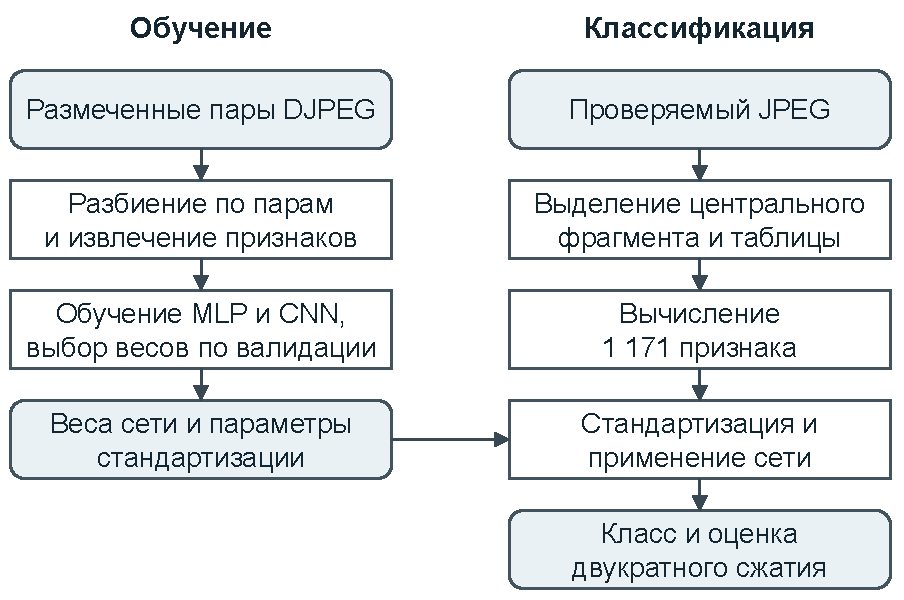
\includegraphics[width=0.86\linewidth]{images/detector-structure.drawio.pdf}
  \caption{Подготовка модели и классификация нового JPEG-файла}
  \label{fig:structure}
\end{figure}

Вместе с весами передаются статистики обучающей выборки. Благодаря этому одинаковое значение признака преобразуется одинаково при обучении и при обработке нового снимка. Для каталога модель загружается один раз, после чего каждый файл проходит ту же обработку, что и при одиночном запуске.

\section{Подготовка размеченных данных}

В наборе DJPEG фрагменту исходного снимка соответствуют два файла с общим идентификатором. Один файл получен после первого сохранения, другой --- после второго~\cite{park2018,djpeg_dataset}. Единицей разбиения служит пара. Так обе версии одного фрагмента всегда остаются вместе.

Алгоритм дополнительно объединяет соседние идентификаторы фрагментов в группы по 1\,000 номеров. Сначала группы случайно распределяются между обучающей, валидационной и тестовой частями. Затем внутри каждой части выбираются полные пары. В итоговом списке сохраняются путь, класс, номер фрагмента и принадлежность к выборке. Для отделения точных копий используются контрольные суммы декодированных пикселей. В архиве отсутствуют идентификаторы полноразмерных фотографий. Разные фрагменты одного снимка могут оказаться в разных выборках.

\section{Извлечение признаков}

Пусть ширина и высота снимка равны $W$ и $H$ пикселям. Из яркостной компоненты выделяется фрагмент $256\times256$ с координатами левого верхнего угла
\begin{equation}
  x_0=8\left\lfloor\frac{W-256}{16}\right\rfloor,\qquad
  y_0=8\left\lfloor\frac{H-256}{16}\right\rfloor.
  \label{eq:crop}
\end{equation}
Такое округление смещает границу центрального фрагмента к ближайшей предшествующей границе блока. Масштаб изображения сохраняется.

Фрагмент содержит $32\times32=1\,024$ блока размером $8\times8$. Из яркости каждого отсчёта вычитается 128, затем для каждого блока вычисляется двумерное ортонормированное ДКП. Используются первые девять переменных составляющих при зигзагообразном обходе матрицы коэффициентов. Для каждой из девяти позиций собираются значения из всех 1\,024~блоков. Постоянная составляющая $(0,0)$ в признаки не входит.

Каждое значение $c$ заменяется целым числом $\lfloor c+0{,}5\rfloor$. Для чисел от $-60$ до~60 предусмотрен отдельный интервал гистограммы. Ещё два интервала собирают значения ниже и выше этих границ. Число отсчётов в каждом интервале делится на 1\,024. Сумма 123 относительных частот одной гистограммы равна единице. Коэффициенты здесь рассчитаны по декодированным пикселям, поэтому при построении гистограммы учитывается и округление яркости при декодировании JPEG.

Девять гистограмм дают $9\times123=1\,107$~признаков. К ним добавляются 64~шага из таблицы квантования яркости, каждый делится на 255. Для каждого из $1\,171$ признаков применяется стандартизация по формуле
\begin{equation}
 \widetilde{x}_j =
 \frac{x_j-\mu_j}{\max(\sigma_j,\,1/1\,024)}.
 \label{eq:scale}
\end{equation}
Здесь $\mu_j$ и $\sigma_j$ --- среднее и стандартное отклонение признака~$j$ по обучающей выборке. Нижняя граница знаменателя равна вкладу одного блока в гистограмму и ограничивает усиление редких признаков.

\section{Архитектуры и обучение моделей}

Персептрон принимает весь вектор из 1\,171~значения. Его скрытые полносвязные слои содержат 64 и 32~нейрона. После каждого скрытого слоя применяется функция $\operatorname{ReLU}(z)=\max(0,z)$. Выходной слой формирует два числа --- оценки до нормировки для класса~0 и класса~1. Персептрон имеет 77\,154 обучаемых параметра.

В свёрточной сети гистограммы образуют девять входных каналов. Фильтр перемещается вдоль оси интервалов, поэтому один и тот же набор весов может обнаружить локальный пик в нескольких частях распределения. Длины ядер двух свёрток равны 5 и~3, число выходных каналов --- 16 и~32. Дополнение нулями сохраняет длину оси интервалов после каждой свёртки. За функцией ReLU следует усреднение соседних отсчётов с окном и шагом~2. Длина уменьшается со 123 до~61, затем до~30.

\begin{figure}[htbp]
  \centering
  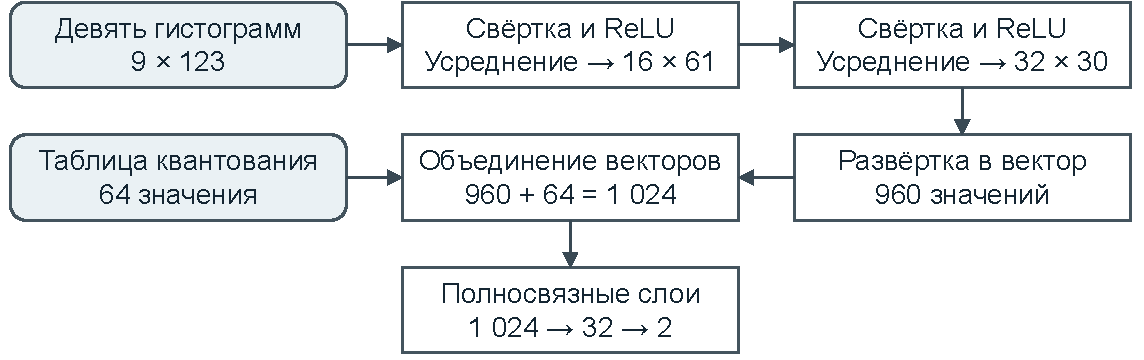
\includegraphics[width=0.98\linewidth]{images/histogram-cnn.drawio.pdf}
  \caption{Преобразование гистограмм и присоединение таблицы квантования в CNN}
  \label{fig:cnn}
\end{figure}

Как показано на рисунке~\ref{fig:cnn}, свёрточная ветвь даёт $32\times30=960$ значений. Вместе с 64~элементами таблицы квантования они поступают на полносвязный слой из 32~нейронов с функцией ReLU. Выходной слой, как и у MLP, содержит два нейрона. Всего в CNN 35\,170 обучаемых параметров.

Пусть $p_{i,y_i}$ --- оценка, которую сеть после нормировки softmax присвоила истинному классу $y_i$ для примера~$i$. Обе сети обучаются по кросс-энтропии. Для пакета из $m$ примеров функция потерь имеет вид
\begin{equation}
 L=-\frac{1}{m}\sum_{i=1}^{m}\ln p_{i,y_i}.
 \label{eq:loss}
\end{equation}
Чем меньше оценка истинного класса, тем больше вклад примера в потери.

Перед каждой эпохой примеры перемешиваются. Для очередного пакета градиенты функции~\eqref{eq:loss} вычисляются обратным распространением ошибки, затем алгоритм Adam обновляет веса. После эпохи потери вычисляются на валидационной выборке. Если значение стало меньше предыдущего минимума, сохраняются текущие веса. Обучение завершается по достижении предельного числа эпох или после заданного числа эпох без улучшения. Для каждой архитектуры выбирается запуск с минимальной валидационной потерей. То же правило определяет модель для программы.

\section{Классификация изображения}

Пусть $z_0$ и $z_1$ --- выходные значения выбранной сети. Оценка класса двукратного сжатия $s$ вычисляется функцией softmax по формуле
\begin{equation}
 s=\frac{\exp z_1}{\exp z_0+\exp z_1}.
 \label{eq:softmax}
\end{equation}
При $s\geqslant0{,}5$ программа выдаёт класс~1, иначе --- класс~0. Значение $s$ позволяет упорядочить результаты для ручного просмотра. Для неподдерживаемого файла класс и оценка не вычисляются.

\subsection*{Выводы}
Единый алгоритм формирует для обеих сетей девять гистограмм и таблицу квантования. Различие состоит в том, как сети используют соседство интервалов. Пары фрагментов распределяются между выборками до обучения, а параметры стандартизации и веса сохраняются для последующей классификации.

\chapter{Технологический раздел}
\textit{Раздел будет подготовлен.}

\chapter{Исследовательский раздел}
\textit{Раздел будет подготовлен после обучения моделей и проведения измерений.}

\chapter*{ЗАКЛЮЧЕНИЕ}
\addcontentsline{toc}{chapter}{ЗАКЛЮЧЕНИЕ}

Разработана программа для предварительного отбора JPEG-файлов с признаками повторного сжатия. Она принимает фотографию или каталог и выдаёт класс и оценку двукратного сжатия. Программа извлекает яркостной фрагмент и таблицу квантования непосредственно из конечного JPEG.

По результатам анализа опубликованных методов выбрано общее представление изображения для двух классификаторов. На 30\,000~размеченных JPEG обучены многослойный персептрон и одномерная свёрточная сеть. Для применения выбрана свёрточная сеть. На тесте из 5\,000~файлов доля верных ответов составила 80,44\,\% против 78,72\,\% у персептрона. Сеть дала на 92~ложных срабатывания меньше и пропустила на шесть повторно сжатых файлов больше. При загруженной модели медианное время обработки фрагмента $256\times256$ на центральном процессоре составило 0,546~мс.

Эксперимент на 300~отдельных фотографиях UCID определил условия, при которых такой отбор полезен. При совпадающей сетке блоков и повышении качества второго сохранения программа обнаружила 75,33\,\% повторно сжатых файлов. При одинаковых значениях качества полнота составила 1,27\,\%, а после сдвига сетки на четыре пикселя --- 1,21\,\% по всем парам настроек. Поэтому файлы с положительным ответом можно передать на дальнейший анализ, а отрицательный ответ при неизвестной истории обработки оставляет вопрос о повторном сохранении открытым.

\clearpage
\phantomsection
\addcontentsline{toc}{chapter}{СПИСОК ИСПОЛЬЗОВАННЫХ ИСТОЧНИКОВ}
\printbibliography[title={СПИСОК ИСПОЛЬЗОВАННЫХ ИСТОЧНИКОВ}]
\chapter*{ПРИЛОЖЕНИЕ А}
\phantomsection
\addcontentsline{toc}{chapter}{ПРИЛОЖЕНИЕ А. Презентация к защите}

Презентация к защите курсовой работы «Исследование нейросетевых методов обнаружения повторного JPEG-сжатия изображений» состоит из девяти слайдов.


\includepdf[pages=-,landscape=true,pagecommand={\thispagestyle{empty}}]{presentation.pdf}

\end{document}
